\documentclass{template/openetcs_report}
% Use the option "nocc" if the document is not licensed under Creative Commons
%\documentclass[nocc]{template/openetcs_article} 
\usepackage{lipsum,url}
\usepackage{xspace}
\usepackage{graphicx}
\usepackage{fixme}
\usepackage{lscape} 
\usepackage{pgfgantt}
\usepackage{adjustbox}
\usepackage{datetime}
\usepackage{appendix}
\usepackage{enumerate}
\usepackage{tikz}
\usetikzlibrary{arrows,shapes,automata,petri,calc}


%user specified macros


\newcommand{\VV}{Verification \& Validation\xspace}
\newcommand{\vv}{verification \& validation\xspace}

\def\CC{{C\nolinebreak[4]\hspace{-.05em}\raisebox{.4ex}{\tiny\bf ++}}}

\newcommand{\bitwalker}{\mbox{\texttt{Bitwalker}}\xspace}

\newcommand{\poke}{\mbox{\texttt{Bitwalker\_Poke}}\xspace}
\newcommand{\peek}{\mbox{\texttt{Bitwalker\_Peek}}\xspace}
\newcommand{\acsl}{\mbox{\textsf{ACSL}}\xspace}
\newcommand{\isoc}{\mbox{\textsf{C}}\xspace}
\newcommand{\framac}{\mbox{\textsf{Frama-C}}\xspace}
\newcommand{\framacwp}{\mbox{\textsf{Frama-C\slash WP}}\xspace}
\newcommand{\why}{\mbox{\textsf{Why}}\xspace}
\newcommand{\wpframac}{\mbox{\textsf{WP}}\xspace}
\newcommand{\altergo}{\mbox{\textsf{Alt-Ergo}}\xspace}
\newcommand{\qed}{\mbox{\textsf{Qed}}\xspace}
\newcommand{\cvc}{\mbox{\textsf{CVC4}}\xspace}
\newcommand{\z}{\mbox{\textsf{Z3}}\xspace}
\newcommand{\coq}{\mbox{\textsf{Coq}}\xspace}
\newcommand{\cealist}{\mbox{\textsf{CEA LIST}}\xspace}

\newcommand{\inl}[1]{\lstinline[style=inline]{#1}}


%% Requirements.


\newcounter{reqnum}
\setcounter{reqnum}{0}
\newcounter{subreqnum}
\newcounter{subsubreqnum}
\newlength{\partopbuf}
\newlength{\topbuf}

% Automated numbering versions of the macros
\newcommand{\req}[1]{\addtocounter{reqnum}{1} \setcounter{subreqnum}{0}
	\begin{description}\item[{\small\reqt-X-\thereqnum}] #1\end{description}
}

\newcommand{\subreq}[1]{
	\addtocounter{subreqnum}{1} \setcounter{subsubreqnum}{0}
	\addtolength{\leftmargini}{1cm}
	\begin{description}
	\item[\hspace{0.5cm}{\small\reqt-X-\thereqnum.\thesubreqnum}] #1
	\end{description}
	\addtolength{\leftmargini}{-1cm}
}

\newcommand{\subsubreq}[1]{
	\addtocounter{subsubreqnum}{1}
	\addtolength{\leftmargini}{2cm}
	\begin{description}
	\item[\hspace{1cm}{\small\reqt-X-\thereqnum.\thesubreqnum.\thesubsubreqnum}] #1
	\end{description}
	\addtolength{\leftmargini}{-2cm}
}

% Fixed version of the commands
\newcommand{\reqfixed}[3]{\addtocounter{reqnum}{1} \setcounter{subreqnum}{0}
	\begin{description}\item[{\small\reqt-#1-#2}] #3\end{description}
}

\newcommand{\subreqfixed}[4]{
	\addtocounter{subreqnum}{1} \setcounter{subsubreqnum}{0}
	\addtolength{\leftmargini}{1cm}
	\begin{description}
	\item[\hspace{0.5cm}{\small\reqt-#1-#2.#3}] #4
	\end{description}
	\addtolength{\leftmargini}{-1cm}	
}

\newcommand{\subsubreqfixed}[5]{
	\addtocounter{subsubreqnum}{1}
	\addtolength{\leftmargini}{2cm}
	\begin{description}
	\item[\hspace{1cm}{\small\reqt-#1-#2.#3.#4}] #5
	\end{description}
	\addtolength{\leftmargini}{-2cm}	
}

% Citation of the requirement

% Citation of the reference (for markup purpose)
%\newcommand{\refreq}[1]{\textbf{#1}}

% Citation of the reference and text (for markup purpose)
% The purpose of this is to automatically replace the placeholder by the 
% full text. \fullrefreq{R-xxx}{} or \fullrefreq{R-xxx}{blabla} 
% will be replaced by \fullrefreq{R-xxx}{text of the R-xxx requirement} 
%\newcommand{\fullrefreq}[2]{\textbf{#1}: \textrm{#2}}

\def\reqt{R-WP2/D2.6}
\newenvironment{justif}{
	\begin{quote}
	\begin{itshape}Justification. 
}{
	\end{itshape}
	\end{quote}
}
%Uncertain items
\newcommand{\qq}[1]{?`#1?}
%C++
\newcommand{\cxx}{C\nolinebreak[4]\hspace{-.05em}\raisebox{.3ex}{\footnotesize\bf ++}\xspace}




\graphicspath{{./template/}{.}{./images/}}
\begin{document}
\frontmatter
\project{openETCS}

%Please do not change anything above this line
%============================
% The document metadata is defined below

%assign a report number here
\reportnum{OETCS/WP4/D4.1V00.03}

%define your workpackage here
\wp{Work Package 4: ``Validation \& Verification Strategy''}

%set a title here
\title{openETCS Validation \& Verification Plan}

%set a subtitle here
\subtitle{Version 00.03}

%set the date of the report here
\date{June 2013}

%define a list of authors and their affiliation here

\author{Marc Behrens and Hardi Hungar}

\affiliation{DLR\\
  Lilienthalplatz 7\\
  38108 Brunswick, Germany
   \\eMail:\{hardi.hungar,marc.behrens\}@dlr.de }

\author{Stephan Jagusch}

\affiliation{AEbt Angewandte Eisenbahntechnik GmbH\\
Adam-Klein-Str.\ 26\\
90429 N\"urnberg, Germany\\
eMail: Stephan.Jagusch@AEbt.de}
  
% define the coverart
\coverart[width=350pt]{openETCS_EUPL}

%define the type of report
\reporttype{Deliverable}



\begin{abstract}
%define an abstract here

  This document describes strategy and plan of the verification and
  validation activities in the project openETCS. As the goals of the
  project include the selection, adaption and construction of methods
  and tools for a FLOSS development in addition to performing actual
  development steps, differing from the plan for a full development
  project, the plan covers also activities evaluating the suitability
  of methods and tools, and it makes provisions for incorporation of
  V\&V of partial developments which are actually done.

  The overall strategy is to support the design process as specified
  in D2.3 and its partial instantiations within openETCS. In
  accordance with the project approach, V\&V shall be done in a FLOSS
  style, and it has to suit a model-based development. A further main
  consideration shall be to strive for conformance with the
  requirements of the standards (EN~50128 and further). This means
  that the contribution of all activities to a complete verification
  and validation shall be defined and assessed.

  The plan details how to perform \vv for a complete development which
  follows the process sketch from D2.3, so that the result conforms to
  the requirements of the standards for a SIL~4 development. This
  includes a definition of activities, the documentation to be
  produced, the organisation structure, roles, a selection of methods
  and tools, a format for describing design artifacts subject to V\&V,
  and a feedback format for the findings during V\&V.

  As D2.3 gives only a rough description of the development steps and
  not yet a complete list of design artifacts, nor one of methods
  applied and formats to be used, this first version of the V\&V plan
  will also lack detail which will to be added in later revisions as
  these informations become more concrete.

  Besides the usual purpose of \vv activities, namely evaluating and
  proving the suitability of design artifacts, V\&V in openETCS will
  also generate information on the suitability of the methods and tools
  employed. For that purpose, a format for describing methods
  and tools to be used in V\&V and one for summarizing the findings
  about the suitability are defined.

  The plan also contains partial instantiations of V\&V which match
  partial developments that are realised within openETCS.

\end{abstract}

%=============================
%Do not change the next three lines
\maketitle
\tableofcontents
\listoffiguresandtables
\newpage
%=============================

\chapter{Document Control}

\begin{tabular}{|p{4.4cm}|p{8.7cm}|}
\hline
\multicolumn{2}{|c|}{Document information} \\
\hline
Work Package &  WP4  \\
Deliverable ID or doc.\ ref.\ & D4.1\\
\hline
Document title & openETCS Validation \& Verification Plan\\
Document version & 00.03 \\
Document authors (org.)  & Hardi Hungar (DLR), Marc Behrens (DLR),
Stephan Jagusch (AEbt) \\
\hline
\end{tabular}

\begin{tabular}{|p{4.4cm}|p{8.7cm}|}
\hline
\multicolumn{2}{|c|}{Review information} \\
\hline
Last version reviewed & -- \\
\hline
Main reviewers & -- \\
\hline
\end{tabular}

\begin{tabular}{|p{2.2cm}|p{4cm}|p{4cm}|p{2cm}|}
\hline
\multicolumn{4}{|c|}{Approbation} \\
\hline
  &  Name & Role & Date   \\
\hline  
Written by    &  Hardi Hungar & WP4-T4.1 Task Leader  &  June 2013\\
\hline
Approved by & -- & -- & \\
\hline
\end{tabular}

\begin{tabular}{|p{2.2cm}|p{2cm}|p{3cm}|p{5cm}|}
\hline
\multicolumn{4}{|c|}{Document evolution} \\
\hline
00.01 & 11/06/2013 & H. Hungar &  Document creation based on draft by
S. Jagusch\\
\hline
Version &  Date & Author(s) & Justification  \\
\hline  
00.02 & 14.06.2013 & J. Gerlach, H. Hungar &  Completed one
requirement table from draft, added detail to V\&V plan for full dev., \\
\hline  
00.03 & 20.06.2013 & J. Gerlach, H. Hungar & Major revisions and
additions
\\
\hline
\end{tabular}

% The actual document starts below this line
%=============================


%Start here

\mainmatter

\chapter{Introduction}

\section{Purpose}
\label{sec:purpose}

The purpose of this document is to define the \vv activities in the
project openETCS.  

{\it This document describes strategy and plan of the
  verification and validation activities in the project openETCS. As
  the goals of the project include the selection, adaption and
  construction of methods and tools for a FLOSS development in
  addition to performing actual development steps, differing from the
  plan for a full development project, the plan covers also activities
  evaluating the suitability of methods and tools, and it makes
  provisions for incorporation of V\&V of partial developments which
  are actually done.}

\begin{description}
\item[WP4-T1-G:] A useful plan for WP 4, that is, one that defines a
way to achieve the goals of WP 4:
  \begin{description}
  \item[WP4-G1:] Identify and demonstrate methods and tools to handle
    the V\&V of a FLOSS development of the EVC software
  \item[WP4-G2:] Perform as much of V\&V on the DAS2Vs produced in the
    project as possible
  \end{description}
\end{description}

\paragraph{Detailed Goals and Means}
\label{sec:detailed-goals-means}

\begin{description}
\item[WP4-T1-G1:] The plan shall give an overview of and a structure to
  the things required from V\&V for an openETCS (FLOSS-) development.
  \begin{description}
  \item[WP4-T1-M1:] Identifies all (most) of the activities which have
    to be made for a full development according to the standards, in a
    form relevant to the approach of openETCS (FLOSS,
    participants). This may include alternatives.
  \end{description}
\item[WP4-T1-G2:] The plan shall provide a framework into which the V\&V
  activities which will be performed within the project do fit.
  \begin{description}
  \item[WP4-T1-M2-1:] Design formats for collecting information about
    DAS2Vs (V\&V tasks), about the results of V\&V activities, about
    activities of V\&V method and tool development, about the results
    of evaluations of V\&V methods and tools. Sketch how all of the
    information is to be gathered and finally incorporated into the
    final V\&V report (D4.4).
  \item[WP4-T1-M2-2:] Identify potential variants of partial
    implementations of V\&V processes which are likely going to be
    performed within the project. These may be (?should be?) related
    to design activities within the project which produce DAS2Vs.
  \end{description}
\item[WP4-T1-G3:] The plan shall delineate means for V\&V within openETCS
  \begin{description}
  \item[WP4-T1-M3-1:] A partial V\&V process (see WP4-T1-M2 above)
    consists of a set of related DASVs and V\&V steps to be applied to
    them. A V\&V step is described by input and output (result,
    purpose) with V\&V methods and means.
  \item[WP4-T1-M3-2:] The plan will prepare the selection of adequate
    methods and means (tools) by providing evaluation criteria and
    incorporating available evaluation results.
  \item[WP4-T1-M3-2-1:] Definition of an evaluation format for tools
    and methods.
  \end{description}
\item[WP4-T1-G4:] The plan shall incorporate currently available
  information on openETCS development process and means and be
  amendable to future changes and additions.
  \begin{description}
  \item[WP4-T1-M4-1:] Use D2.3 in instantiating the general
    requirements laid down in the standards.
  \item[WP4-T1-M4-2:] Use D2.1 for tools.
  \item[WP4-T1-M4-3:] Identify open points and include delineations
    for things which are useful for a complete V\&V but not yet
    planned or detailed by project activities already performed.
  \end{description}
\end{description}


This document describes which verification and validation activities
are needed for a full FLOSS development of the EVC software. It
describes how the work performed within the project openETCS is to be
organised to contribute to such a task, and how to demonstrate that it
can be realised.

The document is only valid in conjunction with the Quality Assurance
plan [1104G13-QA-plan]. It is supplemented by the safety plan, which
focuses on the safety aspect. Verification and validation play an
important role in the safety case. This document identifies the V\&V
activities which do contribute and refers to the safety plan for
further details on the additional requirements to be met and a precise
statement of what has to be established.

\section{Document Structure}
\label{sec:document-structure}

This document comprises both verification and validation plan, as
these activities share some of their methods and tools, and in some
case are applied to the same design artifacts. Nevertheless, these
activities are intended to be and remain independent.

There are three main issues which make this plan different from an
ordinary V\&V plan for a software to develop. First, openETCS is not
only concerned with the software part of the EVC. As part of the
activities, a semi-formal model for SS~026 is to be developed and to
be verified. As the SS~026 covers parts of the ETCS system beyond the
software, also process steps on the system (not just software) level
are to be performed. And in particular the design does not start with
a clearly defined set of requirements on the software.

As a second point, openETCS will not only do development, but
shall also be concerned with processes, methods and tools with the
goal of being able to propose a complete SIL~4 compliant approach. As
part of this, it has to be defined how to handle verification and
validation. This is done in the sections
addressing a ``full development''. Due to the limited resources of the
project, actually performing such a full development is out of the
project's scope. Instead, only some functions will be implemented, and
only partial lines of development will be realised. V\&V related to
these activities is to be planned in the specific sections dedicated
to  ``openETCS''.  

\section{Plan for Completing this Document}
\label{sec:plan-completing-this}

{\it
\paragraph{Terminology}
\label{sec:terminology}
\begin{description}
\item [DAS2V:] Design Artifact Subject to Verification or Validation
\item[G:] Goal
\item[M:] Means
\item[F:] Finding/Result/Action
\end{description}
}


{\it 
\paragraph{Detailed Goals and Means}
\label{sec:detailed-goals-means}

\begin{description}
\item[WP4-T1-G1:] The plan shall give an overview of and a structure to
  the things required from V\&V for an openETCS (FLOSS-) development.
  \begin{description}
  \item[WP4-T1-M1:] Identify all (most) of the activities which have
    to be made for a full development according to the standards, in a
    form relevant to the approach of openETCS (FLOSS,
    participants). This may include alternatives.
  \end{description}
\item[WP4-T1-G2:] The plan shall provide a framework into which the V\&V
  activities which will be performed within the project do fit.
  \begin{description}
  \item[WP4-T1-M2-1:] Design formats for collecting information about
    DAS2Vs (V\&V tasks), about the results of V\&V activities, about
    activities of V\&V method and tool development, about the results
    of evaluations of V\&V methods and tools. Sketch how all of the
    information is to be gathered and finally incorporated into the
    final V\&V report (D4.4).
  \item[WP4-T1-M2-2:] Identify potential variants of partial
    implementations of V\&V processes which are likely going to be
    performed within the project. These may be (?should be?) related
    to design activities within the project which produce DAS2Vs.
  \end{description}
\item[WP4-T1-G3:] The plan shall delineate means for V\&V within openETCS
  \begin{description}
  \item[WP4-T1-M3-1:] A partial V\&V process (see WP4-T1-M2 above)
    consists of a set of related DASVs and V\&V steps to be applied to
    them. A V\&V step is described by input and output (result,
    purpose) with V\&V methods and means.
  \item[WP4-T1-M3-2:] The plan will prepare the selection of adequate
    methods and means (tools) by providing evaluation criteria and
    incorporating available evaluation results.
  \item[WP4-T1-M3-2-1:] Definition of an evaluation format for tools
    and methods.
  \end{description}
\item[WP4-T1-G4:] The plan shall incorporate currently available
  information on openETCS development process and means and be
  amendable to future changes and additions.
  \begin{description}
  \item[WP4-T1-M4-1:] Use D2.3 in instantiating the general
    requirements laid down in the standards.
  \item[WP4-T1-M4-2:] Use D2.1 for tools.
  \item[WP4-T1-M4-3:] Identify open points and include delineations
    for things which are useful for a complete V\&V but not yet
    planned or detailed by project activities already performed.
  \end{description}
\end{description}
}

{\it
\paragraph{Concrete First Steps (in SCRUM terminology: the backlog)}
\label{sec:concrete-first-steps}
\tbd{outdated---update tbd}
\begin{description}
\item[WP4-T1-S1:] Assess the input material
  \begin{description}
  \item[WP4-T1-S1-1:] Assess sketch of the V\&V plan (partly done)
    \begin{description}
    \item[WP4-T1-F1-1-1:] The current format is .doc
    \item[WP4-T1-F1-1-2:] The plan currently lists mainly the requirements
      on the plan and does not yet detail much of the plan itself.
    \item[WP4-T1-F1-1-3:] 
    \end{description}
  \item[WP4-T1-S1-2:] Assess D2.3 ``Process Definition'' with
    definition of DAS2Vs and V\&V steps
    \begin{description}
    \item[WP4-T1-F1-2-1:] DAS2Vs and \vv steps defined on a high level
    \end{description}
  \item[WP4-T1-S1-3:] Assess D2.9 ``Requirements for \VV''
    \begin{description}
    \item[WP4-T1-F1-3-1:] very high-level, requirements included in
      the appendix for reference in further completion in relevant for
      future steps  
    \end{description}
  \item[WP4-T1-S1-4:] Assess D2.1 (``Report on Existing Methodologies'')
    \begin{description}
    \item[WP4-T1-F1-4-1:] Seems very sketchy
    \end{description}
  \item[WP4-T1-S1-5:] Assess development and V\&V activities planned or
    already on the way for taking them into account in the V\&V plan 
    \begin{description}
    \item[WP4-T1-S1-5-1:] Ask a lot of people (or the right people)
    \item[WP4-T1-S1-5-1-1:] Design a query email (to be backed up by
      phone or personal inquiries) 
    \end{description}
  \item[WP4-T1-S2:] Organize the writing 
    \begin{description}
    \item[WP4-T1-S2-1:] Make a detailed work plan
    \item[WP4-T1-S2-1-1:] Transform the sketch to .tex
    \item[WP4-T1-S2-1-2:] Revise the structure according to what is
      expected to be done - accommodating the info on the process (D2.3
      -WP4-T1-S1-2) and on ongoing activities  (WP4-T1-S1-5). 
    \item[WP4-T1-S2-1-3:] References to the requirements (D2.9 -
      WP4-T1-S1-3) are to be included 
    \item[WP4-T1-S2-1-4:] Tools and methods
    \item[WP4-T1-S2-1-4-1:] Format for evaluation (formulate
      evaluation criteria, D4.1a) 
    \item[WP4-T1-S2-1-5:] Result collection
    \item[WP4-T1-S2-1-5-1:] Sketch all the formats (purpose)
    \item[WP4-T1-S2-1-5-2:] Sketch the process of information collection
      (T4.2 and T4.3 will have to do that) 
    \item[WP4-T1-S2-1-6:] Include section on V\&V plan revision
    \end{description}
  \item[WP4-T1-S2-2:] Find contributors
  \item[WP4-T1-S2-3:] Distribute the work
  \end{description}
\item[WP4-T1-S3:]  Do the work
\end{description}  
}

\section{Background Information}
\label{sec:backgr-inform}

\todo{Further Info, perhaps put the project context here }

\subsection{Definitions}

\paragraph{Verification}

Verification is an activity which has to be performed at each step of
the design. It has to be verified that the design step achieved its
goals. This consists at least of two parts:
\begin{itemize}
\item that the artifacts produced in the step are of the right type
  and contain allthe information they should. E.g., that the SSRS
  identifies all components addressed in SS~026, specifies their
  interfaces in sufficient detail and has allocated the functions to
  the components (this should just serve an example and is based on a
  guess what the SSRS should do)
\item that the artifact correctly implements the input requirements of
  the design step. These typically include the main output artifacts
  of the previous step. ``Correctly implements'' includes requirement
  coverage (tracing). This can and should be supported by some
  tools. Adequacy of such tools depends on things like format
  compatibility, degree of automation, functionality (e.g., ability to
  handle m-to-n relations). Depending on the design step (and the
  nature of the artifacts) different forms of verification will
  complement requirement coverage, with different levels of
  support. The step from SS~026 to the SSRS will mainly consist of
  manual activities besides things like coverage checks. Verifying a
  formal (executable) model against the SSRS can be supported by
  animation or simulation to e.g.\ execute test cases which have been
  designed to check compliance with the SSRS. Even formal proof tools
  may be employed to check or establish properties. Model-to-code steps
  offer far more options (and needs) for tool support. And tools or
  tool sets for unit test will support dynamic testing for requirement
  or code coverage. This may include test generation, test execution
  with report generation, test result evaluation and so on. Also, code
  generator verification (or qualification) may play a role,
  here. Integration steps mandate still other testing (or
  verification) techniques.
\end{itemize}
Summarizing, one may say that verification subsumes highly diverse
activities, and may be realized in very many different forms.

\paragraph{Validation}
%\nocite{*}
Validation is name for the activity by which the compliance of the end
result with the initial requirements is shown. In the case of
openETCS, this means that the demonstrator (or parts of it) are
checked against the SS~026 or one of its close descendants (i.e.,
SSRS), taking also further sources of requirements from operational
scenarios and TSIs into accoutn. This will consist of testing the
equipment according to a test plan derived from the requirements and
detailed into concrete test cases at some later stage. Tool support
for validation will thus mainly concern test execution and evaluation,
perhaps supplemented by test derivation or test management. Ambitious
techniques like formal proof are most likely not applicable here.

Thus, the tool support for validation will not differ substantially
from that for similar verification activities.

One might also consider ``early'' validation activities, e.g.\
``validating'' an executable model against requirements from the
SS~026. These are not mandated by the standards and can per se not
replace  verification of design steps. They may nevertheless be worthwhile
as means for early defect detection.

Further (mostly complementary) information on V\&V can be found in the
report on the CENELEC standards (D2.2).

\chapter{Document Evolution}

The verification and validation plan shall be revised in the course of
the project as the design progresses and gets detailed and experiences
with verification and validation are made. This is in accordance with
the EN~50128, where it is required that the plan shall be maintained
throughout the development cycle.

\begin{description}
\item[V01, T0+13:] First version of the plan
\item[V02, T0+17:] First revision, based on the 1st V\&V interim
  reports on applicability of the V\&V approach to model and
  implementation/code (D4.2.1, D4.2.2)
\item[V03, T0+25:] Second revision, based on the internal reports on
  the applicability of the V\&V approach to prototypes of design
  models and code
\item[V04, T0+36:] Final version as part of the final V\&V report (D4.4) 
\end{description}

\chapter{\VV in the Design Process}
\label{cha:vv-design-process}

\textit{Name the design stages and associated V\&V steps, both for the
ideal development (openETCS vision) and project realisation (where we
end with a demonstrator).}

D2.3 defines the openETCS process on an abstract level. It already
defines the main steps. A slightly more detailed picture than the one
given in D2.3 is given in Fig.~\ref{fig:openETCSProcess}. 

\begin{figure}[htb]
  \centering
  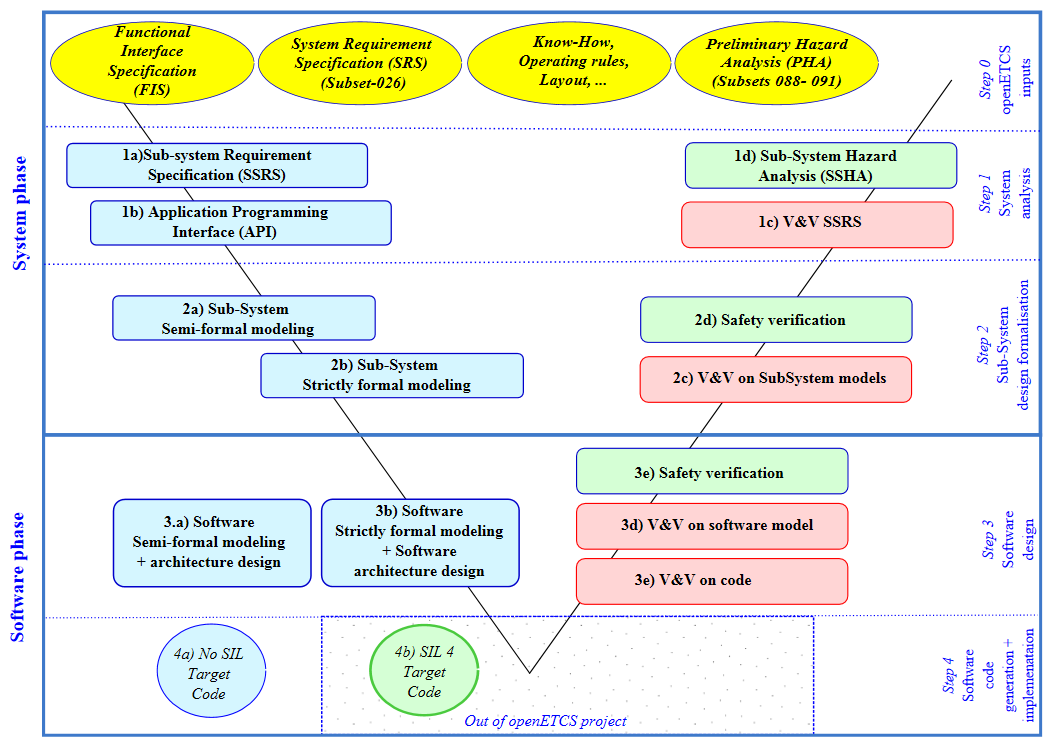
\includegraphics[width=.9\textwidth]{images/ProcessOpenETCS-BeM.png}
  \caption{openETCS Process (rough view)}
  \label{fig:openETCSProcess}
\end{figure}

\textit{The figure needs to be detailed to include all the main design
steps. E.g., the integration activities are subsumed within ``3e) V\&V
on code''. For instance, the integration into the demonstrator should
be made visible. In the end, the figure shall define merely the
``full'' development, this will be of more help than ``openETCS
implementation'' of it. }


\chapter{\VV Strategy}

\texttt{Contributors to this chapter:
  \begin{description}
  \item[DLR] Overall coherence, Safety interface
  \item[All4Tec] aspects of model-based development, FLOSS,
    safety. Mainly in Sec.~\ref{sec:vv-strategy-full} (Full Development).
  \item[SQS] \qq{Contributions to all sections}
  \item[TUBS] Safety interface
  \item[DB, SNCF, NS] Operator role (scenarios, validation goals)
  \end{description}
}

{\it The overall strategy is to support the design process as
  specified in D2.3 and its partial instantiations within openETCS. In
  accordance with the project approach, V\&V shall be done in a FLOSS
  style, and it has to suit a model-based development. A further main
  consideration shall be to strive for conformance with the
  requirements of the standards (EN~50128 and further). This means
  that the contribution of all activities to a complete verification
  and validation shall be defined.  }

\section{\VV Strategy for a Full Development }
\label{sec:vv-strategy-full}



\textit{Here, the ideal shall be described: What we would like to do
  in openETCS but cannot, because we do not know the right methods and
tools yet }

\subsection{Verification Strategy for a Full Development}
\label{sec:verif-strategy-full}



{\it 
Define the strategy for verifying a full devlopment of the EVC software
from the requirements source (ss~026+TSIs+\ldots). This ends with the
verification of the software/hardware integration. The API is
currently the best description of the
interface }

\subsection{Validation Strategy for a Full Development}
\label{sec:valid-strategy-full}

\textit{Classical validation starts after SW/HW integration. Sketch
  how this should look like for the openETCS architecture approach
  (with SSRS and API). Ideal would be a description of how a full
  openETCS EVC software could be taken up by some manufacturer and
  brought to life in a product (validation aspect only, of
  course). Validation will use tests covering operational scenarios.
Not-so-classical validation can start earlier when executable models
become available. If a model can be animated to run an operational
scenario (perhaps with some additional environment/rest-of-system
modeling), design defects may get unveiled before the real validation.}



\section{\VV Strategy for openETCS}
\label{sec:vv-strategy-project}

{\it The project will only perform part of the development, and thus
  also only a part of the V\&V activities. These need to be defined
  and planned, of course.  }

\chapter{\VV Plan for a Full Development}

\texttt{Contributors to this chapter:
  \begin{description}
  \item[DLR] Overall coherence, revise structure of the Verification Report
  \item[All4Tec] Role of model-based testing, \qq{hopefully more}
  \item[SQS] tbd
  \item[CEA] Tools and methods Sec.~\ref{sec:methods-tools})
  \item[U Bremen] Tools and methods (model based testing, bounded
    model checking Sec.~\ref{sec:methods-tools}),
    V\&V process steps
  \item[Fraunhofer] Tools and methods Sec.~\ref{sec:methods-tools})
  \item[TUBS] Safety Interface, general tool list
  \item[TWT, URO] Tools and methods Sec.~\ref{sec:methods-tools})
  \item[DB, SNCF, NS] operator role (end user scenarios, validation
    requirements and contribution)
  \item[Institut Telecom] Methods and Tools Sec.~\ref{sec:methods-tools})
  \end{description}
}

\todo{detail}

{\it
Instantiate the generic \VV plan from the standard (and the draft) to
openETCS. That is, provide the requirements, define the design steps,
identify \vv activities to be performed and documents to be produced.}



{\it
 The plan details how to perform \vv for a complete development which
  follows the process sketch from D2.3, so that the result conforms to
  the requirements of the standards for a SIL~4 development. This
  includes a definition of activities, the documentation to be
  produced, the organisation structure, roles, a selection of methods
  and tools, a format for describing design artifacts subject to V\&V,
  and a feedback format for the findings during V\&V.

  As D2.3 gives only a rough description of the development steps and
  not yet a complete list of design artifacts, nor one of methods
  applied and formats to be used, this first version of the V\&V plan
  will also lack detail which will to be added in later revisions as
  these informations become more concrete.

  Besides the usual purpose of \vv activities, namely evaluating and
  proving the suitability of design artifacts, V\&V in openETCS will
  also generate information on the suitability of the methods and tools
  employed. For that purpose, a format for describing methods
  and tools to be used in V\&V and one for summarizing the findings
  about the suitability are defined.

  The plan also contains partial instantiations of V\&V which match
  partial developments that are realised within openETCS.}

\section{\VV Plan Overview}
\label{sec:plan-overview}

\todo{A list of all steps, with input and output from Jagusch, adapted
to D2.3 steps}

A short overview of the activities (Verification or Validation) which
happen at the respective development steps, to be detailed in the
subsequent sections. The numbering (e.g.\ 2e) refers to
Fig.~\ref{fig:openETCSProcess}.

\begin{description}
\item[SSRS---Verification (1c):] verification that the SSRS the requirements
  consistently extends the requirements base. 
\item[SSRS---Validation (1c):] Deriving a sub-system test specification
\item[SFM---Verification (2c):] Verification that the model formalises
  the requirements
\item[SFM---Validation (2c):] Detailing the test specification,
  perhaps validating the model (e.g.\ via animation)
\item[SW-SFM---Verification (3d):] Verifying the SW-HW architecture
  definition (should be somewhere) and the software model
\item[SW-SFM---Validation (3d):]Perhaps validation of the software model
\item[SW-FFM---Verification (3d):]  verification, employing also
  formal methods/tools 
\item[SW-FFM---Validation (3d):] validation, may e.g.\ employ model checkers
\item[Code---Verification (3e):] verification depends on the code
  generation method (manual, generated, generated with validated
  tool), unit test requirements have to be met, afterwards code
  integration tests
\item[Code---Validation (3e):] no specific activities foreseen
\end{description}

The following steps need some coherent concept. A viable solution
might look simpler / different.  
\begin{description}
\item[EVC Software---Verification (tbd):] Perform software system verification
\item[EVC Software---Validation (tbd):] Validation against user
  requirements/scenarios 
\item[SW/HW integration (tbd):] \qq{Use the API}
\item[Final Validation (tbd):] User requirements and scenarios (based
  on sub-system test specification
\end{description}



\section{Requirements Base}
\label{sec:requirements-base}

The requirements on the EVC software origin in the SS-026 and TSI
specifications.

\todo{detail this, add references}

\section{\VV Methods and Tools }
\label{sec:methods-tools}

{\it The project shall select / develop / describe a chain of methods
  and tools for doing \vv in a full development. Some will be
  suitable for both, \vv, tasks. Each proposal shall be labeled accordingly.}


In common language, the notion {\em ``formal''} is often used in a
broad sense, meaning everything that can be described by rules, even
if they are rather vague.
%
Contrary to that, we use {\em ``formal''} in the narrow sense of
EN-50128 \cite[Section~D.28]{en50128},
meaning strictly mathematical techniques and methods.
%
Since the Aerospace Standard DO-178C \cite{DO-178C}
follows a similar understanding,
but gives more elaborate explanation in its supplementary document
%DO-333 
devoted to formal methods \cite{DO-333},
our presentation closely follows the terminology of the latter.


\begin{quote}
{\em Formal methods are mathematically based techniques for the
specification, development, and verification of software aspects of
digital systems.
%
The mathematical basis of formal methods consists
of formal logic, discrete mathematics, and computer-readable
languages.
%
The use of formal methods is motivated by the expectation
that, as in other engineering disciplines, performing appropriate
mathematical analyses can contribute to establishing the correctness
and robustness of a design.}

\hfill
\cite[Section~1.0, p.1]{DO-333}
\end{quote}

\subsection{Model Based Testing Method}
\subsubsection{Model Based Testing Strategy - generalities}
Testing consists in executing the System Under Test (SUT)
 for some particular inputs and in assessing whether or not the
 corresponding SUT executions conform to some requirements.
 Whatever the testing technique used is, one has to define test cases
 to be submitted to the SUT and associate to them a decision procedure
 called oracle. The oracle allows the tester to compute verdicts according 
to what the executions of SUT (resulting from the test case submission) 
reveal about its correctness.
This correctness is measured with respect to requirements. Model based
 testing is a particular kind of testing technique in which requirements are 
described by models which are executable specifications. Their execution
 traces (or ”traces” for short) are sequences of stimulations of the SUT and
 resulting observations of the SUT reactions. Test cases are sequences of 
stimulations that are selected from the test model. A sequence corresponding
 to an input test data can be obtained by considering a trace of the model and
 ”forgetting” all observations occurring in it. For functional testing, SUT is 
considered as a black bbox: the tester (a human or a test bench) can only
 stimulate the SUT and observe its reactions. Interactions between the tester
 and the SUT result on the definition of traces. Therefore, a SUT can be seen
 as a set of traces that is not known (since SUT is a black box) but the tester
 may discover some of those traces by interacting with SUT. The oracle is based
 on a so called conformance relation. A conformance relation is a mathematical
 relation between the set of traces of the SUT and the set of traces of the model.
 When these sets of traces fulfill the relation we say that the SUT conforms to 
the model. The oracle takes as inputs traces representing an interaction between
 the tester and the SUT and compute verdicts. Whatever the testing techniqu
e is, the set of possible verdicts always contain the verdict Fail which is emitted 
whenever the trace taken as input demonstrates that the SUT does not conform 
to the model. Depending on the testing technique used there may be different 
verdicts emitted when Fail is not emitted. These different verdicts reflect different
 traceability information related to interaction trace taken as input. In this section
 we briefly discuss two model based testing tools that we will use conjointly in the 
OpenETCS project.

\textcolor{magenta}{Start Uni Bremen****\\ }
 The model based testing (MBT) may apply at different level during the
lifecycle:
\begin{itemize}
\item Integration testing
\item (Object) code verification
\end{itemize}
\paragraph{Model-Based System Integration Testing}
The objectives of MBT on system integration level are to
\begin{itemize}
\item validate the correctness and completeness of the development model,
\item verify that the generated code components cooperate correctly on the target HW, in 
order to achieve the system-level capabilities.
\end{itemize}

The first objective implies that the {\it test model} and the original development model are
separate entities; otherwise the system integration test would just validate that all logical
errors still residing in the openETCS development model are really implemented in the code. Even in presence
of a formally validated development model, in which high confidence can be placed, we prefer to create a 
separate test model, because
\begin{itemize}
\item the test model may use a higher level of abstraction since only the SUT behaviour visible at the 
system interfaces is relevant,

\item the test model may specify different interfaces to the SUT, depending on the observable interfaces
in a test suite; the observation level ranges from black-box (only the ``real'' SUT system interfaces
are visible) to grey-box level (some global variables may be monitored or even manipulated by the testing environment, some task or object communications may be observed etc.),  

\item the development model may contain errors that are only revealed during HW/SW integration (for example, calculations failing due to inadequate register word size, or deadlines missed due to insufficient CPU resources).
\end{itemize}
\paragraph{Model-Based Generated Code Testing}
The second application of MBT is for the objective of code verification.
If model-to-text and text-to-text transformations are not formally verified, it
is necessary to verify the outcome of each transformation. Since the transformation
source is a model $M$ (recall that also high-level code is regarded as a model, represented, for example, by its control flow graphs), MBT suites can be derived automatically from this model to show that the
generated code conforms to $M$. 

Observe that in contrast to system-level MBT no redundant model is used for this objective, but the
same model $M$ used for code generation can be used: we just have to verify the consistency between 
code and $M$, without validating $M$'s correctness and completeness. The latter task is separately performed
by means of 
\begin{itemize}
\item property checking or
\item simulation.
\end{itemize}
The model-based testing (MBT) approach can be used to create test
suites conforming to the highest criticality level of the applicable
CENELEC standards, in order to justify that the generated code is
consistent to its model~\cite{PeleskaVL11Nfm,pel2011a,peleska2009d}.
Furthermore, the generated result may be formally verified against the
model. This formal verification task is easier than proving the
correctness of a generator or compiler as a whole, because now just
one concrete artefact (the generated code) has to be checked against
the transformation source. The theoretical foundations of object code
verification, as well as its proof of concept have been established
in~\cite{Pnueli98}. In
\cite{RSRSChapter2012,DBLP:journals/fac/HaxthausenPK11} these concepts
have been refined and applied to the railway domain.


A main advantage of this approach in comparison to performing V\&V for
generators and compilers is that the latter do not have to be
re-verified after improvements and extensions. Therefore we advocate
the test-based code verification approach to be applied in openETCS
for verifying generated high-level source code or object code of SIL-4
applications. 

\textcolor{magenta}{End Uni Bremen****\\ }


\subsubsection{Model Based Testing applied to Open ETCS V\&V}
According to the previous activity on defining the project process, 
the Open ETCS process is based on 3 main inputs for methodology and 
product lifecycle: the SCRUM methodology, the Model Driven Design and the
 Cenelec software development V cycle.
Traditionally, system requirements are directly translated into formal specifications
 on which verification and proof techniques are applied. The use of formal 
specifications and formal language allows then to derive the models using dedicated
 languages (B for instance) in order to guaranty conservation of properties along 
the design process. The main difficulty in this context is to be sure that the
 interpretation of rules has correctly been captured in the formalized specification
 which is not easy to check by the regulators. For this reason, the model based testing
 has been chosen as testing and verification technique within the V\&V activities of
 the OpenETCS project. 

\textcolor{magenta}{Start Uni Bremen****\\ }
Moreover, we suggest to create test models on the basis of the ETCS standard (subset 026) and
the existing high-level test suites made available in subset 076. The latter test cases should 
be feasible computations of the test model, so that the test model really creates a {\it superset}
of the existing test suite from subset 076.

\textcolor{magenta}{End Uni Bremen****\\ }

This technique application will be explained in the following
 paragraphs through the description of different model-based testing tools: 
MaTeLo, Diversity and RT-tester. 



\subsubsection{Matelo Model Based Testing solution}
MaTeLo purpose is to generate test cases for systems whose expected usage and 
behavior are described by a probabilistic model. MaTeLo tool is based on its own test
 model called "usage model" and uses, among other characteristics, usage profiles for 
test case generation. This usage model describes the possibilities regarding the use of 
the soft (in our case; operating scenario) during its whole lifecycle. This usage model is
 performed thanks to a Matelo specific modeler, it allows to generate test cases that will 
then be plugged to the SUT which will be the software semi-formal model realized in the 
frame of WP3 activities.
MaTeLo has three main functionalities: test modeler, test cases generator and test campaign
 analyser. Even if MaTeLo is mainly a test case generation tool, we can consider that this
 tool performs also analysis for different reasons:
\begin{itemize}
\item A test model can be considered as a development artifact the same way as a system
 model for example. So analysis on it could identify some ambiguous or erroneous points in
 test model (i.e. in the future test campaign) or in the specifications (because MaTeLo mode
l is built from system specifications).
\item Even whether test campaign analysis is mainly based on testing activities, analysis
 techniques have to be used as wellThe limit between a model to perform test and a model
 to perform analysis is not so obvious.
\end{itemize}

Because its test case generation is based on a model, MaTeLo belongs to the family of
 Model-Based Testing solutions. MaTeLo model basically uses Markov Chains to describe 
the test model of the SUT implemented for "Black Box Testing" in all xIL steps (MIL, SIL, PIL, HIL).
MaTeLo Usage Model edition facility allows for implementing test models that describe the use
 cases of the SUT completed with the tester point of view, and then, Matelo testing facility 
can generate automatically the test cases generated by the tool.
Thanks to the numerous validation steps, MaTeLo Test Campaign Analysis provides information
 such as test coverage (requirements, model) or reliability of the SUT.
Once the MaTeLo test model is performed and the testing strategy is defined with MaTeLo profiles
 faciulities, MaTeLo generates test cases. For that, MaTeLo Testor contains several test generation 
algorithms that can be used for different purposes. Different test case generators are based on a
 Usage profile approach, considering the occurrence probability of each model transition. Other are
 deterministic (most probable execution path, or all the transitions are covered). 
In the case of Open ETCS project, the SUT model is an on-board EVC, designed according to the 
SRS Subset 026. This specification itself is not sufficient to cover all functional aspects, and tests 
depend strongly on the operating rules to be considered on the observed track. The principle 
for the MaTeLo model would be to encompass all the possible states and transitions that can 
be considered in a well-defined perimeter (based on Subset026, signaling and exploitation
 rules to consider). Then, the test could be precisely defined by the usage profile to adapt 
it to a track oriented testing campaign.

\subsubsection{Diversity Model Based Testing solution}
DIVERSITY is a model based testing tool developed at CEA LIST. Its underlying technology is symbolic
 execution. Symbolic execution has been first defined for programs. The goal of this technique is
 to identify, for each possible execution of the program, the constraints to be satisfied in order to 
follow it. The main idea consists in executing the program, not for concrete numerical values but for 
symbolic parameters, and to characterize constraints on these parameters at each step of the execution.
 In that sens, DIVERSITY is a white box testing tool.
In the frame of the openETCS project we plan to use DIVERSITY to extract test cases from models 
defined in the first phases of the system design. Our goal is to extract test cases dedicated to
 abstract safety requirements. More precisely we focus on safety requirements dealing with 
communication between sub systems. For that purpose we will use the language of sequence 
diagrams extended with timing constraints to specify such requirements. With sequence diagrams,
 one may describe execution scenarios in terms of partially ordered message passing between 
subsystems. Message passing can be structured thanks to operators expressing sequencing, 
parallelism, choice, loop...  
It is possible to automatically analyze sequence diagrams with DIVERSITY in order to extract test
 cases. The originality is that, thanks to projection mechanisms, it is possible to extract test cases,
 not only for the entire system, but also for any sub systems composing it. Because of this mechanism, 
sub systems can be tested as soon as they are implemented, even though the entire system is 
not yet implemented. In such a process we perform a particular kind of unitary testing in which 
unit test cases are built according to the usage that will be made of the sub system in the entire
 system. In the frame of OpenETCS, this functionality could be useful in order to realize the unitary
 and modular tests.
The first step consists in defining a requirement model in the form of a sequence diagram or a
 Matelo Test scenario. The requirement model is analyzed with DIVERSITY in step 2. This analysis 
results on a so-called symbolic tree, who’s each path denotes a possible (symbolic) execution of
 the sequence diagram. Such trees may be theoretically infinite due to the possible occurrences
 of the "loop" operator of sequence diagrams. Therefore, DIVERSITY uses various stopping 
criteria to stop the computation (typically based on message coverage notions). 
The symbolic tree computed in step 2 characterizes executions of the whole system model. 
However, because testing the whole system may be complicated in terms of testing architecture, 
or simply because one wants to test some sub systems before the whole system is implemented, 
we offer a mechanism to extract symbolic trees for each distinguished sub system. This is based 
on so-called projection techniques. This operation is realized in step 3. In step 4, each identified 
sub system is tested thanks to a real time off-line testing algorithm.
Then, we can relate correctness of sub systems and correctness of the whole system by using a 
compositionality theorem.
The compositionality theorem expresses that, the conformance of each subsystems to all their 
projections guarantees the conformance of the whole system to the sequence diagram. A direct
 consequence is that any faults of the whole system can be discovered as a fault of at least one
 of its sub systems. This implies that testing the whole system mainly comes to test each of its 
sub systems after a short test integration phase testing that each sub system is correctly connected.
 We believe that such an approach will be very useful for ETCS systems which are by nature very 
distributed and thus hardly observable and controllable as a whole. The share of OBU EVC kernel
 in sub-system is the role of the SSRS model, and this refinement to diversity will be possible once
 this functional decomposition of the EVC will be released.

\subsubsection{Complementary use of the DIVERSITY and MaTeLo}
The use of the two tools can be done in a complementary way that would 
allow a more efficient test case set generation. 
MaTeLo would start from the test model, and generate automatically all the
 use cases that can be encountered in CBTC use. MaTeLo tool analyses the 
models as black box, and generates tests according to a stochastic approach. 
DIVERSITY will analyze these scenarios, based on a symbolic execution of the 
semi-formal SysML model (white box testing), in order to filter the tests generated
 by MaTeLo and to reduce the test case set.
As discussed in previous Sections, the two tools DIVERSITY and MaTeLo handle 
different kinds of models. The version of DIVERSITY that we will use in the project 
handles high level models in the form of sequence diagrams. Such models can be used 
to specify requirements on communication scenario between subsystems of a reference
 system under test. Models handled in MaTeLo are automata labeled by transfer functions
 and probabilities. Such models are useful to describe executable behaviors very close to
 the actual implementation, and based on operating scenarii. Clearly these two levels of 
modeling are useful in design processes of safety critical applications such as ETCS implementations,
 and can be combined in different ways for improving the test coverage of our EVC Software kernel.
 Indeed, ETCS systems have such a level of complexity, that it is difficult to describe them in a model
 straight from the requirements. Therefore, the refinements provided by two modeling levels are very
 helpful. Moreover, it is mandatory to maintain a good traceability between these two levels of modeling, 
in order to fulfill the safety requirements.
The complementarity of these tools takes place in some refinement processes in which high level 
requirements can be implemented into executable models. However, it is crucial to assess whether 
executable models correctly implement requirements. In practice this may be a difficult question
 because it requires to efficiently explore the executable model, which by nature is generally 
huge because it represents in a precise manner the functional behaviors of the actual implementation.
 In order to overcome this problem we plan to take benefits from the fact that executable 
models of ETCS will be described in the form of communicating executable models. This fact permits
 to see the model as a collection of communicating subsystems. This permits to take benefits of the 
compositional result described in the Diversity, and use it for white box testing (the internal behavior
 of functional modules and blocks defined in the kernel can then be precisely tested)..


\subsubsection{The RT-tester} 
\textcolor{magenta}{Start Uni Bremen****\\ }
The RT-Tester test automation tool, made by Verified
\cite{verified_website}, performs automatic test generation, test
execution and real-time test evaluation.  It supports different
testing approach such as unit testing, software integration testing
for component, hardware/software integration testing and system
integration testing.  The RT-Tester version  follows the
model-based testing approach \cite{Peleska2011} and
it provides the following features :
\begin{itemize}
\item Automated Test Case Generation 
\item Automated Test Data Generation 
\item Automated Test Procedure Generation 
\item Automated Requirement Tracing 
\item Test Management system 
\end{itemize}
Starting from a test model design with UML/SYML, the RT-tester fully
automatically generates test cases. They are then specified as test
data (sequences of stimuli with timing constraints) and used to
stimulate the SUT and run concurently with the generated test
oracles. The test procedure is the combination of the test oracles and
the SUT that can be compiled and executed.

The tool supports test cases/data generation for structural
testing. It automatically generates  reach statement coverage, branch coverage and
modified condition/decision coverage (MC/DC) as far as this is possible.
The test cases may all be linked to requirements ensuring a complete
requirement traceability. 
Additionally RT-tester may produce test cases/data from a LTL
formula, since a LTL formula describes a possible run of the model.

Taking advantage of SysML requirements diagram, the test cases and
test procedures are directly linked to the requirements. It is then
possible to perform test campaign guided by requirements.

Finally the tool may produce the documentation of tests for
certification purposes. For each test cases the following document are
produced :
\begin{itemize}
\item {\em Test procedure}: that specifies  how one test case can be
  executed, its associated test data produced and how the SUT
  reactions are evaluated against the expected results.
\item {\em Test report}: that summarizes all relevant information
  about the test execution.
\end{itemize}

In \cite{brauer_efficient_2012}, a general approach  on how to qualify
model-based testing tool according to the standard ISO 26262 ad RTCA
DO178C has been proposed and applied with success to the RT-tester
tool. Following the same  approach compatibility with the CENELEC EN50128
may be easily done. 

\textcolor{magenta}{End Uni Bremen****\\ }
\subsection{Characterisation of Formal Methods}

Based on rigorous mathematical notions, formal methods may be used
to describe software systems' requirements in an unambiguous way,
thus supporting precise communication between engineers.
%
Formally specified requirements can be checked for consistency and
completeness by appropriate tools;
also, compliance between different representation levels of
specification can be verified.
%
Formal methods allow one to check software properties like:

\begin{itemize}
\item Freedom from exceptions
\item Freedom from deadlock
\item Non-interference between different levels of criticality
\item Worst case resource usage (execution time, stack, \ldots)
\item Correct synchronous or asynchronous behaviour,
        including absence of unintended behaviour
\item absence of run-time error
\end{itemize}


In order to subsume this variety of applications under a single
paradigm,
the DO-178C
considers a formal method to consist in applying a
formal {\em analysis} to a formal {\em model}.
%
Both analysis and model differs depending on the particular method.
%
For most methods, the model
is just identical to the source code; however, it may
also be e.g.\ a tool-internally generated abstract state space (used
in the Abstract Interpretation method, cf.\
Section~\ref{sec:Abstract Interpretation} below).
%
For most methods, analysis tools need human advice;
however, they may also be fully automatic (e.g.\ for 
Abstract Interpretation or Model Checking, cf.\
\ref{sec:Model Checking}).

\subsection{Formal Analysis Methods}
\label{sec:formal-analysis}

In this section we present
the three most common methods for formal analysis.
The foundation of these analysis
methods are well understood and they have been
applied to many practical problems.


\subsubsection{Abstract Interpretation}
\label{sec:Abstract Interpretation}

The abstract interpretation method
\cite{Cousot.Cousot.1976}
builds at every point of a given program a conservative\footnote{
        i.e.\ guaranteeing soundness
}
abstraction
of the set of \emph{all} possible states that may occur there
during any execution run. Such a representation is also called an 
\emph{over-approximation}, in the sense that it captures all possible
concrete behaviours of the program, while the abstraction might lead to 
consider states that cannot occur in a concrete execution.
%
Abstract interpretation 
determines particular effects of the program relevant for the
properties to be analysed, but does not actually execute it.
%
This allows one to statically determine dynamic properties of
infinite-state programs.
%
The main application is to check the absence of runtime errors, like
e.g.\ dereferencing of null-pointers, zero-divides,
and out-of-bound array accesses.
%
While conventional ad-hoc static analysis tools such as PCLint or \mbox{QA\cxx}
are well-tailored for quick, but incomplete analyses,
abstract-interpretation based tools while requiring more computation time, are
\emph{safe} in the sense that they guarantee that {\em all} potential
runtime errors are detected. On the other hand, such a tool might report 
spurious warnings, related to states that are included in the abstraction but
do not correspond to concrete executions. Such \emph{false alarms} can be
avoided to some extent by increasing the precision of the 
abstraction~\cite{Souyris.Delmas.2007},
at the expense of the computation time of the analysis. However,
%
human intervention is often required to improve the approximation accuracy
w.r.t.\ those program points where {\em false alarms}
have to be removed.


\subsubsection{Deductive Verification}
\label{sec:deduct-verif}
Deductive methods
\cite{Beckert.Marche.2010}
\cite{Ledinot.Pariente.2010}\nocite{Beckert.Marche.2010}
perform mathematical proofs to establish formally specified properties
of a given program, thus providing rigorous evidence. Its primary use is to
verify functional properties of the program.
This method is based on the Hoare logic~\cite{Hoare.1969,Hoare.Wirth.1973},
or axiomatic semantics, in
which functions are seen as predicate transformers. In summary, a function
\texttt{f}
is given a state described by a given predicate $P$ and transforms 
it into a new state, described by another predicate $f(P)$.
In this context, the specification of \texttt{f} is given by a \emph{contract}, 
which defines the predicate $R$ that \texttt{f} requires from its callers and
the predicate $E$ that it ensures upon return. Verifying the implementation
against such a specification amounts to proving that for each $P$ such that
$P\Rightarrow R$ (i.e.\ that satisfies the requirement of \texttt{f}), then
$E\Rightarrow f(P)$ 
(i.e.\ the concrete final state is implied by what \texttt{f} ensures).

%
Tools based on deductive verification usually extract proof obligations 
from program code and property specifications and attempt to 
prove them, either automatically or interactively. Some tools are tightly
coupled to a given theorem prover, while other such as Why3~\cite{why3} 
promote a cooperation across a wide range of provers.
%
In addition to the contracts of the function, it is often required to provided
additional annotations in order to be able to use deductive verification. In
particular, for each loop in the code, a suitable \emph{loop invariant} has
to be provided. A loop invariant is a property that is true when encountering
the loop for the first time and, if true at the beginning of a loop step, stays
true at the end of this step. From both hypotheses, it is then possible to
inductively conclude that the invariant is true for any number of step, and in
particular at the end of the loop. While it is possible to synthesize
automatically loop invariant in some simple cases, in particular thanks to
abstract interpretation, this activity must most of the time be done manually.

Similarly, some proof obligations are too complicated to be handled by automated
theorem provers, and must be discharged interactively via proof
assistants~\cite{coq,isabelle}. Deductive verification is thus much less
automated than abstract interpretation. On the other hand, it is much more
flexible for functional properties verification, in the sense that it can be
used to prove any property that can be expressed in the specification language
of the tool (usually any first-order logic property), while abstract
interpretation is limited to the properties that fit within the abstract setting
that has been chosen.

\subsubsection{Model Checking}
\label{sec:Model Checking}

Model checking
\cite{Clarke.Schlingloff.2001}\nocite{Robinson.Voronkov.2001}
explores all possible behaviours of a program to
determine whether a specified property is satisfied.
%
It is applicable only to programs with reasonable small state spaces;
the specifications are usually about temporal properties.
%
If a property is unsatisfied, a counter-example can be generated
automatically,
showing a use case leading to property violation.


\subsection{Verification with Formal Methods}

In the railway domain, the standard
EN~50128 highly recommends use of formal methods in
requirements specification (\cite[Table A.2]{en50128}),
software architecture (A.3),
software design and implementation (A.4),
verification and testing (A.5),
data preparation (A.11), and
modelling (A.17)
for Safety Integrity Level SIL~3 and above.
%
However, functional\slash black-box testing is still mandatory in
verification; this constraint may be considered as discouraging from
the use of formal methods.

Until recently, the situation was quite similar in the aerospace
domain.
%
J.\ Joyce, a member of the RTCA
standardisation committee SC-205, described
Airbus' problems in certifying their ``unit-proof for unit-test''
approach:

        \begin{quote}
        ``{\em Formal methods were used for certification credit in
        development of the A380, but apparently it was not a trivial
        matter to persuade certification authorities that this was
        acceptable even with the reference to formal methods in
        DO-178B as an alternative method.}''
        \end{quote}


Such experiences eventually caused the more detailed treatment of
formal method issues in the revision C of DO-178 that appeared in
late 2011.
%
The DO-178C considers formal methods as special cases of
reviews and analyses; thus incorporating them without major
structural changes of the software development recommendations.
%
For an employed formal method, the standard requires to justify its
unambiguity, its soundness\footnote{
        i.e., that the method never asserts a property to be true
        when it actually may be not true
},
and any additional assumptions\footnote{
        e.g.\ data range limits
}
needed by the method.
%
The DO-178C admits formal property verification on object code
as well as on source code, the latter additionally needing
evidence about property preservation of the source-to-object
code compiler.
%
However, ``{\em functional tests
executed in target hardware are always required to ensure that the
software in the target computer will satisfy the high-level requirements}''
\cite[FM.12.3.5]{DO-333}.

As a consequence of subsuming formal methods under general reviews and
analyses, no deviating special rules to qualify tools are necessary:
``{\em
Any tool that supports the formal analysis should be assessed under
the tool qualification
guidance required by DO-178C and qualified where necessary.}''
\cite[FM.1.6.2]{DO-333}.
Of course, for the railway domain, the rules of EN~50128 for supporting
software tools and languages must be taken into account
\cite[Section~6.7]{en50128}.

During the last 15 years, formal methods have grown out of academic
playgrounds and become practically relevant in several applications
domains.
Below, we sketch a few different tools, also to indicate the variety
of issues formal methods can be applied for.
Many of the tools mentioned below provide formal verification for programs
written in~C.
There is currently insufficient support for the programming language~\cxx,
which is predominantly used in Thales' RBC product.
%
A list of free software tools for formal verification
can be found at \cite{gulliver}.
%
The list is not meant to be complete.
%
It is structured by tool purpose, and each tool is briefly
introduced.

\subsubsection{The Frama-C Source Code Analysis Suite}
\label{sec:Frama-C}

{\em Frama-C}~\cite{Cuoq.2012} is a suite of tools 
from CEA LIST and INRIA Saclay, dedicated to the analysis of C source code.
Frama-C gathers several static analysis techniques in a single
collaborative framework. Frama-C also features a formal specification language,
ACSL~\cite{ACSL}, in which the contract of each function of the program can
be written (see section~\ref{sec:deduct-verif}), as well as assertions that
are supposed to hold at a given program point.

Frama-C's kernel as well as many analysis plug-ins are available under the
LGPL Open-Source licence from~\cite{frama-c}. Other plug-ins have been
developed by third-party developers, either in an academic~\cite{Bouajjani.2011}
or an industrial~\cite{Ledinot.Pariente.2010} background. The remainder of this
section only deals with the plugins that are released with Frama-C's kernel and
are the most relevant for OpenETCS.

\paragraph{Value Analysis} 
Value analysis is based on abstract interpretation 
(section~\ref{sec:Abstract Interpretation}). This plugin analyses a
complete application, starting from a given entry point, and gives at
each program point an over-approximation of the values that can appear
in each memory location at this point. For each operation, Value also
checks that whether the abstract value of the operands guarantees that
the operation is safe. If this is not the case, it emits an alarm, in
the form of an ACSL assertion, and attempts to reduce its abstract
state to represent only safe concrete values. If all concrete values
are unsafe, then either the corresponding branch of the code is dead
(and was only taken because of the over-approximation), or there is a
real error in the code. Otherwise, the analysis resumes with the
reduced state. Conversely, if no alarm is emitted by Value, the
analysed code is guaranteed not to lead to a run-time error.

Value can also be used to check whether ACSL annotations hold or
not. However, it is restricted to the subset of the ACSL language that
fits well within the abstract representation that is used.

Finally, Value can be tweaked in various ways to increase the
precision of the results (leading to fewer false alarms), generally at
the expense of the computation time and amount of memory used by the
analysis. These options are described in more detail in Value's
reference manual~\cite{frama-c-va}.

\paragraph{WP} 
WP is a plugin dedicated to deductive verification 
(see section~\ref{sec:deduct-verif}). It uses different models 
to represent C memory states in the logic. More abstract models lead to easier
proof obligations, but cannot be used in presence of low-level pointer 
arithmetic, while more concrete ones are able to deal with any C construction,
at the expense of far more complex proof obligations.

WP has two native interfaces to discharge proof obligations. The first one calls
the Alt-Ergo~\cite{alt-ergo} automated theorem prover, while the second let the
user do the proof within the Coq~\cite{coq} interactive proof assistant. In
both cases, the original formulas are first run through an internal simplifier,
that can directly discharge the simplest proof obligations, without the need
for a call to an external tool. In addition, WP can also call the
Why3~\cite{why3} back-end, through which it has access to a
variety of automated provers. Alt-Ergo, Coq and Why3 are available
under Open-Source licences (Cecill-C and LGPL). The various possible settings
of WP are described in its user manual~\cite{WP}.

While WP's primary usage is to prove functional properties expressed as 
function contracts, it can also be used to prove the absence of runtime error,
either by discharging the alarms emitted by Value Analysis, or by generating
proof obligations for all operations that might lead to a runtime error 
(without having to use Value first). The latter case is done through the use
of the \emph{RTE} plugin, that generates an ACSL assertion for each potentially
dangerous operation. WP can then generate proof obligations for these assertions
as usual.

\paragraph{Aoraï}
While Value and WP are used to verify program properties, the Aoraï plugin is
dedicated to generate ACSL specifications (which can then be proved by Value
or WP). More precisely, it takes as input an automaton describing the sequence
of function calls that are allowed during the execution of a program (from a
given entry point). From that automaton, Aoraï instruments the code and provides
ACSL contract for each function so that if all the contracts hold, then the
code is behaving according to the automaton.

Transitions of the automaton can be guarded by conditions over the state of the
program at a given call point. Full syntax of Aoraï's input language is 
described in~\cite{aorai}.




\subsubsection{The Diversity Symbolic Execution Tool}


DIVERSITY is a symbolic execution tool developed at $CEA-LIST$. Its underlying technology is {\em symbolic execution}.  Symbolic execution has been first defined for programs \cite{King75,Clarke,Rama}. The goal of this technique is to identify, for each possible execution of the program, the constraints to be satisfied in order to follow it.  
The main idea consists in executing the program, not for concrete numerical values but for symbolic parameters, and to characterize constraints on those parameters at each step of the execution. 
For instance let us consider that at a given step of an execution the next instruction $ins$ to be executed is $if(x>14) x:=x+1$. Moreover let us suppose that from the previous steps we have computed a couple $(x\rightarrow a, a<45)$ meaning that before the execution of $ins$, the  value of $x$ is represented by the symbolic parameter $a$, with the constraint that $a<45$. Executing $ins$ results on a new context $(x\rightarrow a+1 , a<45 \land a>14)$ taking into account both the constraints so that the instruction is executable ($x$ has to be greater than $14$ and since $x$ value is $a$ it means that $a$ has to be greater than $14$) and the variable updates induced by the instruction (the result of the execution of $x:=x+1$ is that $x$ value is now $a+1$). $a<45 \land a>14$ is called a {\em path
  condition}. Generating test data to follow some executions comes the to use solvers to find values satisfying such path conditions. 
Symbolic execution has been later adapted to modeling formalisms like {\em Input Output Symbolic Transition Systems} (\cite{RGLG03,GAL00}), later to timed version of Input Output Symbolic Transition Systems (\cite{EGL11,BEGL12}) and also to various industrial modeling languages like the {sequence diagrams} of the $UML$ (\cite{BGS11}). Those symbolic execution adaptations have been used in model based testing contexts. System under test are compared to their models by means of two conformance relations namely {\em $ioco$} (\cite{Tre96a}) and its timed extension {\em $tioco$} (\cite{Kri04}). Those two conformance relations are among the most widely accepted conformance relations. Several testing algorithms were defined based on those conformance relations (\cite{GLRT06, EGL11, BEGL12}).

In the frame of the openETCS project we plan to use DIVERSITY to extract test cases from models defined in the first phases of the system design. Our goal is to extract test cases dedicated to abstract safety requirements. More precisely we focus on safety requirements  dealing with communication between sub systems. For that purpose we will use the language of sequence diagrams extended with timing constraints to specify such requirements. With sequence diagrams, one may describe execution scenarios in terms of partially ordered message passing between subsystems. Message passing can be structured thanks to powerful operators expressing sequencing, parallelism, choice, loop...   
In \cite{BGS11} we show how to automatically analyze such sequence diagrams with DIVERSITY in order to extract test cases. The originality is that is that, thanks to projection mechanisms, it is possible to extract test cases, not only for the entire system, but also for any of its distinguished sub systems. Thanks to this mechanism, sub systems can be tested as soon as they are implemented, even though the entire system is not yet implemented. In such a process we perform a particular kind of unitary testing in which unit test cases are built according to the usage that will be made of the sub system in the entire system. 
Faults identified with such an approach are very relevant because we know that they will be activated in the system. The process is illustrated in Figure \ref{ct}.
The first step consists in defining a requirement model in the form of a sequence diagram. The requirement model is analyzed with DIVERSITY in step $(2)$. This analysis results on a so-called {\em symbolic tree}, whose each path denotes a possible (symbolic) execution of the sequence diagram. 
Such trees may be theoretically infinite due to the possible occurrences of the "loop" operator of sequence diagrams. Therefore, DIVERSITY uses various stopping criteria to stop the computation (typically based on message coverage notions). 
The symbolic tree computed in step $(2)$ characterizes executions of the whole system model. However because testing the whole system may be complicated in terms of testing architecture, or simply because one wants to test some sub systems before the whole system is implemented, we offer a mechanisms to extract symbolic trees for each distinguished sub system. This is based on so-called {\em projection} techniques (\cite{FGG07,EGL11}). This operation is realized in step $(3)$. In step $(4)$ Each identified sub system is tested thanks to a real time off-line testing algorithm (\cite{BEGL12}).
Thanks to a compositionality theorem (\cite{bannour2012}) we can relate correctness of sub systems and correctness of the whole system (see step $5$).
The compositionality theorem expresses that, the conformance of each subsystems to all their projections guarantees the conformance of the whole system to the sequence diagram. A direct consequence is that any faults of the whole system can be discovered as a fault of at least one of its sub systems. This implies that testing the whole system mainly comes to test each of its sub systems regardless of a very simple test integration phase in which one only tests that each sub system is correctly connected. We believe that such an approach will be very useful for ETCS systems which are by nature very distributed and thus hardly observable and controllable as a whole. We plan to identify with experts how to partition them into several sub systems that will be more easily observable and controllable at the testing phase.  


\begin{figure}
\centering
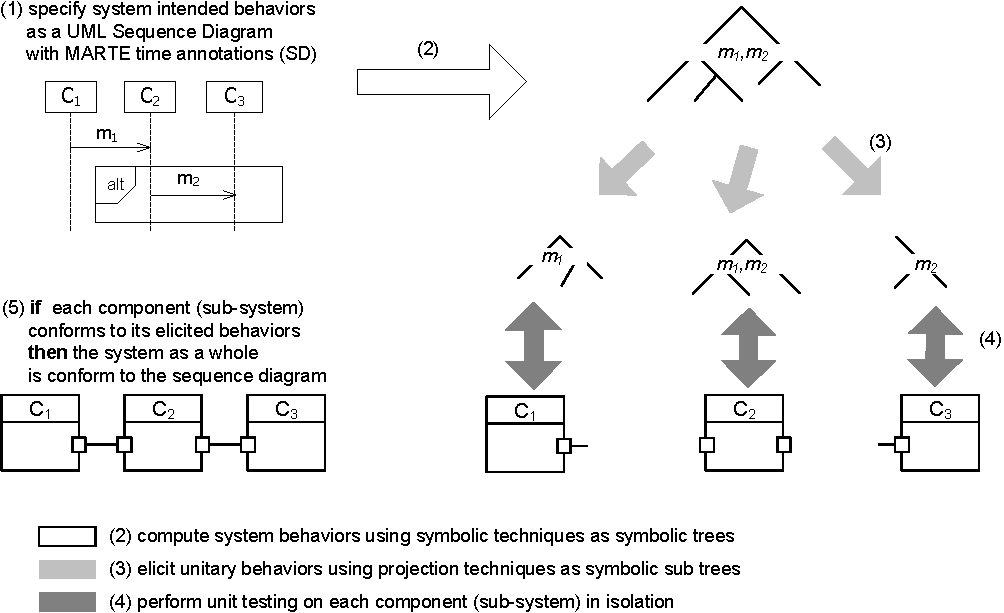
\includegraphics[scale=0.525]{approach_3.pdf}
\caption{\label{ct}Compositionnal Testing}
\end{figure}








\subsubsection{Microsoft's Verifier for Concurrent C (VCC)}

VCC is a tool from Microsoft Research
to prove correctness of annotated concurrent C programs.
It was mainly developed to verify Microsoft's \emph{Hyper-V} hypervisor.
%
It supports an own annotation language providing
e.g.\ contracts, pre- and postconditions, and type invariants.
%
It uses the Boogie tool to generate proof obligations,
and the automatic prover Z3 to prove them.
%
If an obligation is violated, the Model Viewer tool can generate a
counter-example use case.
%
VCC is available for non-commercial use from \cite{vcc}.


\subsubsection{The Proof Assistants Coq and Isabelle}


{\em Coq} is an interactive theorem prover and proof checker,
developed at INRIA, and based on
higher-order logic and the natural deduction calculus.
%
It provides the formal language {\em Gallina}, in which
mathematical definitions can be expressed as well as
executable algorithms and theorems.
%
The supporting tool for tactics-based semi-interactive development of
proofs is available from \cite{coq}.
%

{\em Isabelle}, maintained at Cambridge University,
and its predecessor {\em HOL}\footnote{
        Higher Order Logic
},
are similar tactic-oriented interactive theorem provers.
%
Isabelle is available from \cite{isabelle}.
%
While Isabelle is not yet supported in the Frama-C environment,
Coq is.


\subsubsection{The Model Checker NuSMV}

{\em SMV}\footnote{
        Symbolic Model Verifier
}
has been the first model checker based on binary decision
diagrams.
%
{\em NuSMV} is a reimplementation by the Fondazione Bruno Kessler
that is in addition capable of
performing SAT-based model-checking.
%
It supports both
Linear Temporal Logic (LTL) and Computation Tree Logic (CTL).
%
NuSMV's source code is available under an LGPL license from
\cite{nusmv}.


\subsubsection{Formal Verification of Real-Time Aspects based on Timed Automata}

Verifying system properties involving time is difficult with traditional model checking methods. Commonly used \emph{temporal logics}, such as LTL or CTL catch discrete and qualitative aspects of time and allow to formulate properties such as\footnote{The prefixes are the corresponding linear time operators.}
\begin{itemize}
  \item[\bf X] At the next point in time a property holds.
  \item[\bf F] At some future point in time a property holds.
  \item[\bf G] Always/generally (now and at any future point in time) a property holds.
  \item[\bf U] A property $p$ holds until a property $q$ holds.
\end{itemize}

While it is possible to state properties that must be satisfied at individual (discrete) points in time, continuous and quantitative aspects of time as in the safety requirement
\begin{quote}
``The delay between receiving an emergency message and the issuing of a brake order is less than 1 second.''
\end{quote}
are a real challenge. The problem does not stem from discrete vs. continuous time, as any physical realisation of a real-time system is inherently discretised by its clock. Instead, an operator for expressing arbitrary temporal quantities or differences is missing. Thus, for LTL and a clock of 1 kHz, it would be required to use the operator \textbf{X} 1000 times. This notation is rather unhandy, as it enforces to express a functional property relative to a particular system.


This lack of expressivity is not merely a matter of notation, i.e., LTL or CTL, but also of the underlying semantics. Before introducing a better suited logic we will first consider a formalism that serves as this logic’s semantics -- namely \emph{timed automata}.

\paragraph{Timed Automata}

Timed automata \cite{Alur1994} are essentially finite automata extended with a finite set of clocks that all proceed at the same rate. Clocks may be individually reset to zero. Clock variables can be part of constraint expressions that may be used as transition guards. A transition can only be taken if its guard is fulfilled. Similarly, it is possible to specify an invariant for a state that must be satisfied when the automaton is in this state. Thus, we can enforce time constraints for the runs of the automaton.

\paragraph{An Example}
The timed automaton in Figure~\ref{fig:ta:emergency1} depicts an automaton representing an over-simplified version of an OBU subsystem processing emergency messages. It has three states, one clock $x$ and three actions, \textit{emg\_msg} (reception of an emergency message), \textit{proc\_msg} (processing the message, e.g. raising an alarm) and \textit{brake} (issueing the brake order). Upon receiving an emergency message the clock $x$ is reset. The \textit{proc\_msg}-transition is guarded by the clock constraint $x<1$ preventing the transition to be taken if $x\geq 1$. The same holds for the \textit{brake}-transition. 

\begin{figure}
\begin{center}
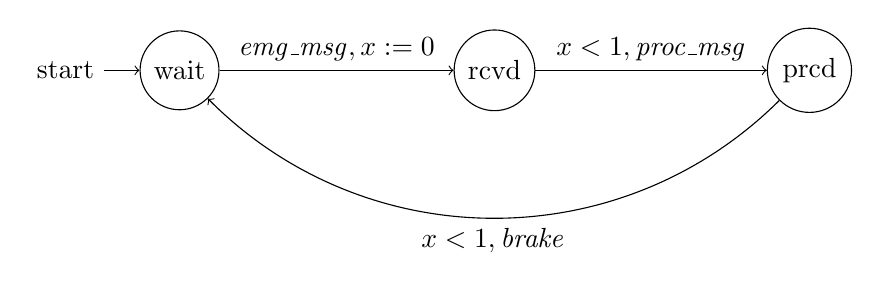
\begin{tikzpicture}[node distance=1.3cm,bend angle=45,auto]
\node [state, initial] (s1) at (0,0) { wait };
\node [state] (s2) at (4,0) { rcvd };
\node [state] (s3) at (8,0) { prcd };
\path[->] (s1) edge node {$\mathit{emg\_msg}, x:=0$}(s2);
\path[->] (s2) edge node {$x<1, \mathit{proc\_msg}$}(s3); 
\path[->] (s3) edge [bend left] node {$x<1, \mathit{brake}$}(s1);
\end{tikzpicture}
\end{center}
\caption{First (faulty) version of a timed automaton for processing emergency messages}
\label{fig:ta:emergency1}
\end{figure}

One might think that the automaton from Figure~\ref{fig:ta:emergency1} thus fulfills the safety requirement stated above. Due to the operational semantics of timed automata this is not true: a timed automaton in a given state can either take a transition or wait for an arbitrary amount of time. Thus, if automaton waits in state rcvd and $x$ exceeds one second, the system will deadlock as the next transition is guarded by the constraint $x<1$. A run of the automaton that could serve as counterexample is, e.g.

$$(\mathrm{wait},0)\rightarrow(\mathrm{wait},0.5)\rightarrow(\mathrm{rcvd},0.5)\rightarrow(\mathrm{rcvd},2)\rightarrow\textrm{DEADLOCK}$$

A solution to this problem is to force the automaton to proceed by placing \emph{progress} constraints on the states. This has been done in Figure~\ref{fig:ta:emergency2}. The transition guards have been omitted as they are not necessary anymore. Now the safety property ``The delay between receiving an emergency message and the issuing of a brake order is less than 1 second.'' is fulfilled.

\begin{figure}
\begin{center}
\small
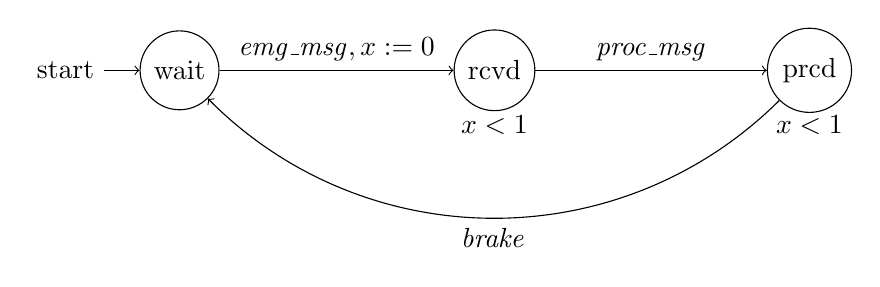
\begin{tikzpicture}[node distance=1.3cm,bend angle=45,auto]
\node [state, initial] (s1) at (0,0) { wait };
\node [state] (s2) at (4,0) { rcvd }; 
\node [state] (s3) at (8,0) { prcd };
\node at (4,-0.7) {$x<1$};
\node at (8,-0.7) {$x<1$};
\path[->] (s1) edge node {$\mathit{emg\_msg}, x:=0$}(s2);
\path[->] (s2) edge node {$\mathit{proc\_msg}$}(s3); 
\path[->] (s3) edge [bend left] node {$\mathit{brake}$}(s1);
\end{tikzpicture}
\end{center}
\caption{Corrected version of the timed automaton for processing emergency messages}
\label{fig:ta:emergency2}
\end{figure}

\paragraph{UPPAAL}

\textsc{Uppaal} is a tool for modelling and verifying timed automata developed by the universities of Uppsala and Aalborg \cite{UppaalTutorial04}. This toolkit is under constant development and comes with an academic as well as a commercial licence. Moreover, there is a comparably large body of literature featuring \textsc{Uppaal}, providing introductory and industrial examples. 

\textsc{Uppaal} extends timed automata with synchronisation enabling concurrent, communicating automata representing different parts of a system. In addition, variables other than clocks are supported making the modelling language more powerful. The logic used for expressing real-time properties is a subset of TCTL (Timed Computation Tree Logic). Nesting of temporal operators is not supported leading to a restriction in expressiveness.

\paragraph{From SysML/UML to Timed Automata}

Timed automata and statecharts in SysML/UML are both based on the concept of finite automata. Thus, it is reasonable to extract timed automata from existing statecharts which is addressed in the literature \cite{David2002, Knapp2002, Jensen2004}. In this way, safety properties -- formalised as TCTL formulae -- can be verified in an automated fashion for a given statechart.

\textcolor{red}{To be continued}



\subsection{Simulation-based Approaches}

\subsubsection{Simulation with SystemC}






\section{Verification for a Full Development}
\label{sec:verif-full-devel}

\textit{for each of the verification steps identified in the plan
  overview, the following has to be instantiated: }
\subsection{DASV Verification}
\label{sec:dasv-verification}

\subsubsection{Task}
\label{sec:dasv-verif-task}

\subsubsection{Documents to Be Produced}
\label{sec:dasv-verif-docum-be-prod}

\subsubsection{Phase Specific Activities}
\label{sec:dasv-verif-phase-spec-activ}

\subsubsection{Techniques and Measures}
\label{sec:dasv-verif-techniques-measures}

\textit{Here the verfication plan begins}

\subsection{SSRS Verification (1c)}
\label{sec:ssrs-verification}

\subsubsection{Task}
\label{sec:ssrs-verif-task}

The SSRS (sub-system requiement specification) outlines the subsystem
which is going to be modeled within the project. The SSRS describes
the architecture of the subsystem (functions and their I/O) and the
requirements allocated to these functions. If necessary, the
requirements are rewritten in order to address the I/O and to
correspond to the allocation. It also provides the classification into
vital and non vital requirements and data
streams. The architecture part is described in a semi-formal language,
and the requirements are described in natural language.

The SSRS is to be viewed as a supplement to the SS-026 and the
TSIs and is not intended to replace them. The verification has to
check that a complete and consistent set of functionalities have been
identified and that the architecture is adequate. 

\todo{Verifiy hazard analysis too?}


\subsubsection{Documents to Be Produced}
\label{sec:ssrs-verif-docum-be-prod}

SSRS verification report.

\subsubsection{Phase Specific Activities}
\label{sec:ssrs-verif-phase-spec-activ}

\subsubsection{Techniques and Measures}
\label{sec:ssrs-verif-techniques-measures}

 Due to the informal
nature of the SSRS, mainly manual techniques are to be applied.

\qq{Review}



\subsection{SFM Verification (2c)}
\label{sec:sfm-verif-verification}

\subsubsection{Task}
\label{sec:sfm-verif-task}

\subsubsection{Documents to Be Produced}
\label{sec:sfm-verif-docum-be-prod}

\subsubsection{Phase Specific Activities}
\label{sec:sfm-verif-phase-spec-activ}

\subsubsection{Techniques and Measures}
\label{sec:sfm-verif-techniques-measures}




\todo{further verification phases}



\section{Structure of the Verification Report}
\label{sec:structure-vv-plan}

\tbd{the following is a draft which is to be adapted to the }
{\it
The verification and validation plan covers the following central topics:
\begin{description}\setlength{\parsep}{0pt}\setlength{\itemsep}{0pt}\setlength{\topsep}{0pt}
%\reqfixed{04}{040}{x}
%\subreqfixed{04}{040}{1}{x}
\item[Header] containing all information to identify, this report, the
  authors, the approbation and reviewing entities.
\item[Executive Summary] giving an overview of the major elements from
  all sections. 
\item[Problem Statement] describing the challenges to be answered by
  \VV as well as the decisions to be taken based on the V\&V results
  as well as how to cope with potentially faulty output. It further
  describes the accreditation scope based on the risk assessment done
  on V\&V-level. 
\item[V\&V Requirements Traceability Matrix] links every V\&V artifact
  back to the requirements to measure e.g. test coverage and to
  directly link V\&V results to the requirements. 
\item[Acceptability Criteria,] describing the criteria for acceptance
  of the artifact into the \VV process e.g. as the direct translation
  of the requirements into metrics to measure success, are used
  e.g.\ for burndown charts within the process. 
\item[Assumptions] that are identified during the design of the
  verification and validation strategy and how these assumptions have
  an impact on the verdict by listing capabilities and limitations. 
\item[Risks and Impacts] that come across the execution of V\&V tasks
  together with the impacts foreseen. 
\item[V\&V Design] states how the V\&V process builds up including
  data preparation, execution and evaluation. 
\item[V\&V Methodologies] giving a step-by-step walkthrough of all
  possible V\&V activities including the assumptions, and
  verdict-relevant limitations and criteria for, e.g.,  model
  verification, model-to-code verification, unit testing, integration
  testing and final validation (according to the standard, this
  involves running the software on the target hardware).  
\item[V\&V Issues] describing unsolved V\&V issues and their impact on
  the affected proof or verdict. 
\item[Peer Reviews] going into details on how the community can take
  part and how official bodies and partners are integrated into the
  development and review process. 
\item[Test Plan Definition] going into the details of testing by
  describing among other things: 

\begin{description} 
\item[Title] as a unique identifier to the test plan.
\item[Description] of the test and the test-item giving information
  about version and revision. 
\item[Features] to be tested and not to be tested in combination are
  listed together with information background.  
\item[Entry Criteria] which have to be met by the EVC before a test
  can be started, e.g. that the EVC has to be in level~3 limited
  supervision with the order to switch to level~2. 
\item[Suspension criteria and resumption requirements] are the central
  key to a smooth automation of the tests covering topics like
  \emph{when exiting this test before step 10, which entry criteria
    does it comply to or which resumption sequence has to be executed
    to continue testing}. 
\item[Walkthrough] covering a step-by-step approach of the test plan.
\item[Environmental requirements] going into the details of what is
  needed concerning the test environment, e.g. tools, adapter, data
  preparation. 
\end{description}

\item[Discrepancy Reports] identifying the defects.
\item[Key Participants] describing the assignment and task for each
  role involved.  

\begin{description}
\item[Accreditation of Participants] describing who was accredited to
  which role during the \VV phase. 
\item[V\&V Participants] listing the partners participating in V\&V activities,
\item[Other participants] including other interest groups such as
  reviewer by affiliate partners\footnote{affiliate partners are
    non-funded companies who signed the project cooperation agreement
    and with it get read access to the repositories starting from
    incubation phase to contribute e.g. by reviewing}. 
\end{description}

\item[Timeline] giving the timeline for the baselines as input to the
  V\&V process and identifying when each artifact should be created. 
\end{description}
}


\section{Validation for a Full Development}
\label{sec:valid-full-devel}

\textit{for each of the validation steps identified in the plan
  overview, the following has to be instantiated: }
\subsection{DASV Validation}
\label{sec:dasv-validation}

\subsubsection{Task}
\label{sec:dasv-valid-task}


\subsubsection{Documents to Be Produced}
\label{sec:dasv-valid-docum-be-prod}


\subsubsection{Phase Specific Activities}
\label{sec:dasv-valid-phase-spec-activ}

\subsubsection{Techniques and Measures}
\label{sec:dasv-valid-techniques-measures}



\subsection{SFM Validation (3d)}
\label{sec:sfm-validation}

\subsubsection{Task}
\label{sec:sfm-valid-task}

The formalisation of the reqauirements in form of a semi-formal model
enables a systematic check of the completeness and consistency of the
system test specification.

The model itself can perhaps be animated (depending on the concrete
form which is not yet fixed). This offers the chance to an early
(preliminary) validation of the design.

\subsubsection{Documents to Be Produced}
\label{sec:sfm-valid-docum-be-prod}

\begin{enumerate}
\item Revised System Test Specification
\item SFM validation report
\end{enumerate}

\subsubsection{Phase Specific Activities}
\label{sec:sfm-valid-phase-spec-activ}

\tbd{}

\subsubsection{Techniques and Measures}
\label{sec:sfm-valid-techniques-measures}

\tbd{}

\subsection{Final Validation (tbd)}
\label{sec:final-validation}

\subsubsection{Task}
\label{sec:final-valid-task}

The final validation shall ascertain that the end result of the
development---the EVC software in its specified environment---behaves
as required. 

\subsubsection{Documents to Be Produced}
\label{sec:final-valid-docum-be-prod}

\begin{enumerate}
\item System Test Definition (based on System Test Specification)
\item System Validation Report
\end{enumerate}

\subsubsection{Phase Specific Activities}
\label{sec:final-valid-phase-spec-activ}

Testing the software against the user requirements.

\subsubsection{Techniques and Measures}
\label{sec:final-valid-techniques-measures}

\qq{Testing in a validated testbed (including API animation/simulation)}


\section{Implementation of \VV}
\label{sec:implementation-vv}

The \vv has to be performed in cooperation with WP~3, which
produces DAS2Vs (models and code), and with WP~7, where methods
and tools are defined and developed. 

To exchange information with WP~3, formats are needed for collecting
information about DAS2Vs (V\&V tasks) and for giving back information
about the results of V\&V activities. Similarly, with WP~7
communication shall use formats to describe V\&V methods and tools
(input from WP~7) and the results of evaluations of V\&V methods and
tools.

\todo{Formats, activity organisation}


\chapter{\VV Plan for openETCS}

\texttt{Contributions to this chapter
  \begin{description}
  \item[DLR] overall coherence, lab test description
  \item[U Bremen] RT Tester application, \qq{more}
  \item[Siemens] Application story (to be detailed)
  \item[SQS] tbd
  \item[CEA] Application story (to be detailed)
  \item[All4Tec] Application story (to be detailed)
  \item[DB, SNCF, NS] Validation requirements
  \end{description}
}

\todo{Describe how to proceed in openETCS to achieve the most. Include
all partial V\&V instantiations with their relation/potential
contribution to a full V\&V.}

{\it
  \begin{itemize}
  \item \vv for partial developments
  \item evaluation
  \item demonstration story of capabilities
  \end{itemize}
}


\section{Verification Plan for openETCS}
\label{sec:verif-plan-open}

\section{Validation Plan for openETCS}
\label{sec:valid-plan-open}





\appendix
\chapter{Requirements on \VV}

\todo{Explain the requirement chapter.}
{\it
  \begin{itemize}
  \item Requirements from D2.9.
  \item Take the lists from the draft from 121207, retain the structure (at
    least preliminarily). 
  \end{itemize}
}

\section{Requirements on \VV from D2.9}
\label{sec:requirements-vv-D29}
\todo{Adapt the intro text} 

The already provided requirements require a
safety plan compliant to the CENELEC EN~50126, 50128 and 50129.  This
pulls a number of requirements on V\&V, including Verification and
Validation plans. On the topic of compliance to EN~50128, one shall
also refer to the D2.2 document.


\reqfixed{02}{061}{A Verification plan shall be issued and complied
  with.}  
\subreqfixed{02}{061}{01}{The verification plan shall
  provide a method to demonstrate the requirements covering all the
  development artifacts.}  
\subreqfixed{02}{061}{02}{The verification
  plan shall state all verification activities required for each of
  these development artifacts.} 
 \reqfixed{02}{062}{A Validation Plan
  shall be issued and complied with.}  
\subreqfixed{02}{062}{01}{The
  validation plan shall provide a method to validate all functional
  and safety requirements over all development artifacts.}
\subreqfixed{02}{062}{02}{The validation plan shall state all
  validation activities required for each of these development
  artifacts.}

\reqfixed{01}{021}{The test plan shall comply the mandatory documents
  of the SUBSET-076, restricted to the scope of the OpenETCS project.}
\begin{justif}
  It will possibly be difficult to model all the tests in the course
  of the project, but the test plan should at least be complete.
\end{justif}


\reqfixed{02}{063}{Each design artifact needs a reference artifact
  which it implements (\emph{e.g.} code to detailed model, SFM to SSRS
  model\dots)} 

\subreqfixed{02}{063}{01}{The implementation between them relation
  shall be specified in detail.}  e.g.\ for state machine and a higher
level state machine mapping of interfaces, states and transition is
required.  This includes additional invariants, input assumptions and
further restrictions. This informaiton is the basis for verification
activities.

\subreqfixed{02}{063}{02}{The design of the artifacts shall be made
  such to allow verifiability as far as possible.}

\reqfixed{02}{064}{The findings from the verification shall be traced,
  and will be adequately addressed (taken into consideration, or
  postponed or discarded with a justification).}



\section{General Requirements on Verification}

\tbd{Reformulate text taken from the EN~50128 to avoid copyright infringements.}
{\footnotesize\sffamily\centering
  \begin{longtable}{||p{.15\textwidth}|p{.4\textwidth}|p{.4\textwidth}||}
    \hline\hline
    \bfseries Excerpt from EN~50128:2011 [N01] & \bfseries
    Requirement & \bfseries Project Relevance\\
    \hline\hline
    \endhead
    \hline\hline
    \endfoot
    5.3.2.7 & For each document, traceability shall be provided in
    terms of a unique reference number and a defined and documented
    relationship with other documents.  &
    fully applicable\\
    \hline 5.3.2.8 & Each term, acronym or abbreviation shall have the
    same meaning in every document.  If, for historical reasons, this
    is not possible, the different meanings shall be listed and the
    references given.  &
    \\
    \hline 5.3.2.9 & Except for documents relating to pre-existing
    software (see 7.3.4.7), each document shall be written according
    to the following rules:
    \begin{itemize}
    \item it shall contain or implement all applicable conditions and
      requirements of the preceding document with which it has a
      hierarchical relationship;
    \item it shall not contradict the preceding document.
    \end{itemize}
    &
    \\
    \hline 5.3.2.10 & Each item or concept shall be referred to by the
    same name or description in every document.  &
    \\
    \hline 6.5.4.14 & Traceability to requirements shall be an
    important consideration in the validation of a safety-related
    system and means shall be provided to allow this to be
    demonstrated throughout all phases of the lifecycle.  &
    \\
    \hline 6.5.4.15 & Within the context of this European Standard,
    and to a degree appropriate to the specified software safety
    integrity level, traceability shall particularly address
    \begin{enumerate}[a)]
    \item traceability of requirements to the design or other objects
      which fulfil them,
    \item traceability of design objects to the implementation objects
      which instantiate them.
    \item traceability of requirements and design objects to the tests
      (component, integration, overall test) and analyses that verify
      them.
    \end{enumerate}

    Traceability shall be the subject of configuration management.  &
    \\
    \hline 6.5.4.16 & In special cases, e.g. pre-existing software or
    prototyped software, traceability may be established after the
    implementation and/or documentation of the code, but prior to
    verification/validation.  In these cases, it shall be shown that
    verification/validation is as effective as it would have been with
    traceability over all phases.  & This requirement does not apply to
    the project.
    \\
    \hline 6.5.4.17 & Objects of requirements, design or
    implementation that cannot be adequately traced shall be
    demonstrated to have no bearing upon the safety or integrity of
    the system.  &
    \\
    \hline
\end{longtable}}


{\footnotesize\sffamily\centering
  \begin{longtable}{||p{.15\textwidth}|p{.8\textwidth}||}
    \hline\hline
    \textbf{Excerpt from EN~50128:2011 [N01]} & \textbf{Requirement} \\
    \hline\hline
    \endhead
    \hline\hline
    \endfoot
    6.1.4.1 & Tests performed by other parties such as the
    Requirements Manager, Designer or Implementer, if fully documented
    and complying with the following requirements, may be accepted by
    the Verifier.
    \\
    \hline 6.1.4.2 & Measurement equipment used for testing shall be
    calibrated appropriately.  Any tools, hardware or software, used
    for testing shall be shown to be suitable for the purpose.
    \\
    \hline 6.1.4.3 & Software testing shall be documented by a Test
    Specification and a Test Report, as defined in the following.
    \\
    \hline 6.2.4.2 & A Software Verification Plan shall be written,
    under the responsibility of the Verifier, on the basis of the
    necessary documentation.
    \\
    \hline 6.2.4.3 & The Software Verification Plan shall describe the
    activities to be performed to ensure proper verification and that
    particular design or other verification needs are suitably
    provided for
    \\
    \hline 6.2.4.4 & During development (and depending upon the size
    of the system) the plan may be sub-divided into a number of child
    documents and be added to, as the detailed needs of verification
    become clearer.
    \\
    \hline 6.2.4.5 & The Software Verification Plan shall document all
    the criteria, techniques and tools to be used in the verification
    process.  The Software Verification Plan shall include techniques
    and measures chosen from Table A.5, Table A.6, Table A.7 and Table
    A.8.  The selected combination shall be justified as a set
    satisfying 4.8, 4.9 and 4.10
    \\
    \hline 6.2.4.6 & The Software Verification Plan shall describe the
    activities to be performed to ensure correctness and consistency
    with respect to the input to that phase. These include reviewing,
    testing and integration.
    \\
    \hline 6.2.4.7 & In each development phase it shall be shown that
    the functional, performance and safety requirements are met.
    \\
    \hline 6.2.4.8 & The results of each verification shall be
    retained in a format defined or referenced in the Software
    Verification Plan.
    \\
    \hline 6.2.4.9 & The Software Verification Plan shall address the
    following:
    \begin{enumerate}[a)]
    \item the selection of verification strategies and techniques (to
      avoid undue complexity in the assessment of the verification and
      testing, preference shall be given to the selection of
      techniques which are in themselves readily analysable);
    \item selection of techniques from Table A.5, Table A.6, Table A.7
      and Table A.8;
    \item  the selection and documentation of verification activities;  
    \item  the evaluation of verification results gained;   
    \item  the evaluation of the safety and robustness requirements;  
    \item the roles and responsibilities of the personnel involved in
      the verification process;
    \item the degree of the functional based test coverage required to
      be achieved;
    \item the structure and content of each verification step,
      especially for the Software Requirement Verification (7.2.4.22),
      Software Architecture and Design Verification (7.3.4.41,
      7.3.4.42), Software Components Verification (7.4.4.13), Software
      Source Code Verification (7.5.4.10) and Integration Verification
      (7.6.4.13) in a way that facilitates review against the Software
      Verification Plan.
    \end{enumerate}
    \\
    \hline
\end{longtable}}

\todo{Insert other tables.}

\section{Glossary}
\label{sec:glossary}

\begin{description}
\item [DAS2V:] Design Artifact Subject to Verification or Validation
\item[EVC] European Vital Computer
\end{description}


\bibliographystyle{unsrt}
\bibliography{bibliography}


\nocite{*}
%===================================================
%Do NOT change anything below this line

\end{document}
